\documentclass[UTF8, 12pt]{ctexart}

\usepackage{amsmath}

\usepackage{geometry}
\geometry{a4paper, scale = 0.95} % a4纸, 版心占页面长度的比例为0.9

\usepackage{enumitem} % itemize, 列表

\usepackage{graphicx}

\begin{document}

	\noindent
	二极管, 符号
\includegraphics[scale = 0.2]{01/二极管符号}

	伏安特性曲线 :

	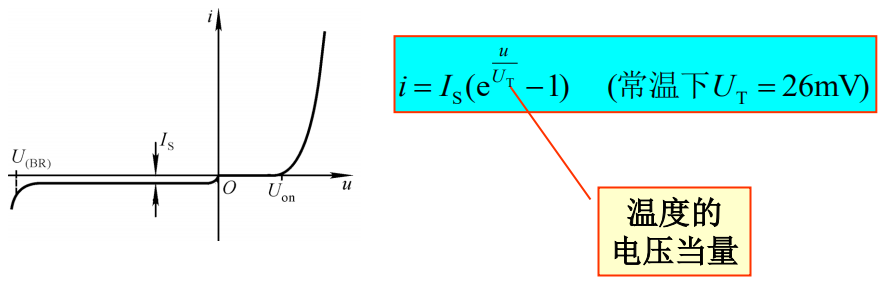
\includegraphics[scale = 0.4]{01/二极管伏安特性.png}

	特性和参数 :
	\begin{itemize}[leftmargin = 4em]
		\item $ 0 < U < U_{on} $, 正向电流为0, $ U_{on} $ 称为开启电压(硅0.5v, 锗0.1v)
		\item $ U < U_{on} $, 出现正向电流, 按照指数规律增长
		\item $ U_{BR} < U < 0 $, 反向电流很小, 称为反向饱和电流 $ I_{s} $
		\item $ U < U_{BR} $, 反向电流急剧增大, $ U_{BR} $ 称为反向击穿电压 
		\item 正向压降 $ U_{F} $, 规定的正向电流下, 二极管的压降(硅0.6 $ \sim $ 0.8v, 锗0.2 $ \sim $ 0.3v)
	\end{itemize}

	简化模型 : 理想二极管(导通时无压降, 截止时无电流), 理想二极管+理想电压源(导通时压降为开启电压), 理想二极管+电压源(导通时伏安特性为线性)

	小信号模型(静态基础上有动态信号作用) : 求静态工作点(去掉动态部分), 二极管等效为 $ r_{d} = \frac{26(mV)}{I_{D}(mA)} $ 的电阻

	多二极管 : 将二极管拿开, 比较正向开路电压大小, 大的先导通, 再分析剩下的(钳位(控制二极管两端电压)/隔离(截止状态隔离两端))

	~

	\noindent
	稳压二极管, 符号
\includegraphics[scale = 0.2]{01/稳压二极管符号.png}

	稳压电路 : 

	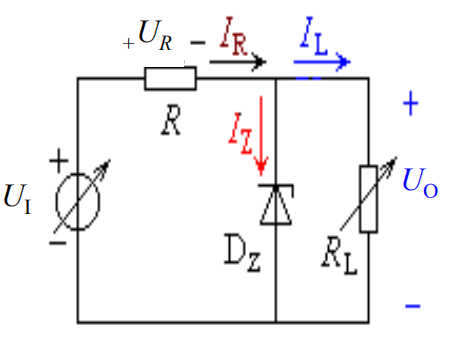
\includegraphics[scale = 0.2]{01/稳压二极管稳压电路.png}

	通过稳压管的电流在一定的范围内, $ R_{L} $ 两端的电压是固定的

	~

	\noindent
	晶体三极管(BJT), 符号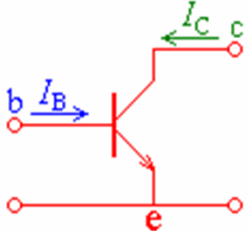
\includegraphics[scale = 0.2]{01/晶体三极管符号.png}(NPN型)

	特性和参数 :
	\begin{itemize}[leftmargin = 4em]
		\item 共基极电流放大系数 $ \alpha $, 三极管放大时, $ I_{C} = \alpha I_{E} $
		\item 共发射极电流放大系数 $ \beta $, 三极管放大时, $ I_{C} = \beta I_{B} $
		\item $ I_{B} + I_{C} = I_{E} $
		\item 饱和区 : 发射结(be)正偏(P的电压大于N), 集电结(cb)正偏
		\item 截止区 : 发射结电压小于开启电压, 集电结反偏
		\item 放大区 : 发射结正偏, 集电结反偏
	\end{itemize}

	输入特性曲线 :

	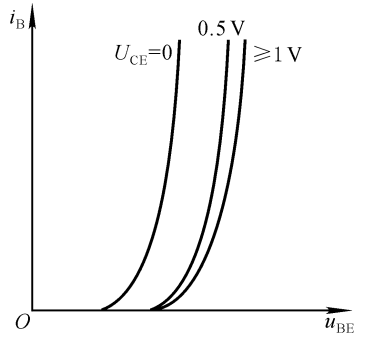
\includegraphics[scale = 0.4]{01/晶体三极管输入特性曲线.png}

	输出特性曲线:

	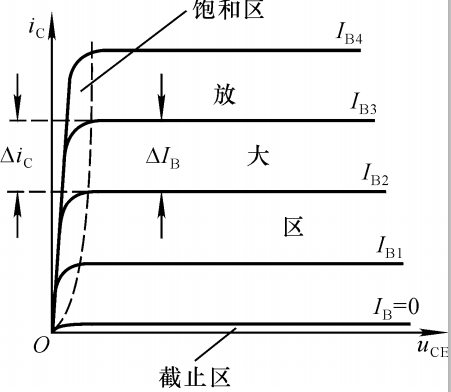
\includegraphics[scale = 0.4]{01/晶体三极管输出特性曲线.png}

	判断三极管状态 : 
	\begin{itemize}[leftmargin = 4em]
		\item 先看发射结, 电压是否大于开启电压, 不大于就是截止
		\item (1). 假设处于放大状态($ U_{BE} = \text{开启电压}, I_{C} = \beta I_{B} $), 计算 $ U_{CE}, U_{CB} $, 集电结反偏就是放大状态
		\item (2). 假设处于临界饱和状态($ U_{CE} = \text{开启电压} $), 算出 $ I_{CS}, I_{BS} $, 和实际 $ I_{B} $ 对比, 如果 $ I_{B} $ 小就是放大状态
		\item 放大状态下, 知道三个脚的电位, 则 : 基极电压为中间值, 发射级电压和基极差(锗管0.2 $ \sim $ 0.3)/(硅管0.6 $ \sim $ 0.7), 剩下的是集电极; $ U_{CE} > 0 $ 为NPN型
	\end{itemize}

	~

	\noindent
	场效应管(FET), 分为结型场效应管(N沟道, P沟道), 符号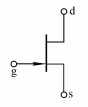
\includegraphics[scale = 0.4]{01/结型场效应管符号.png}, 绝缘栅型场效应管(增强型, 耗尽型, 每一种也分NP沟道), 符号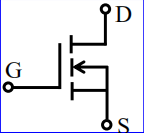
\includegraphics[scale = 0.2]{01/绝缘栅型场效应管符号.png}(箭头朝里表示N沟道, 虚线表示增强型, 实线为耗尽型)

	结型场效应管的输出特性曲线 :

	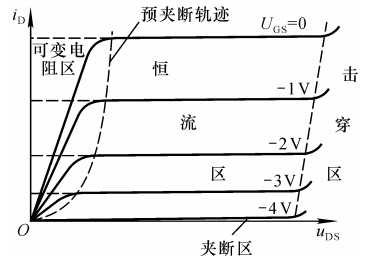
\includegraphics[scale = 0.4]{01/结型场效应管输出特性曲线.png}

	结型场效应管的转移特性曲线 :

	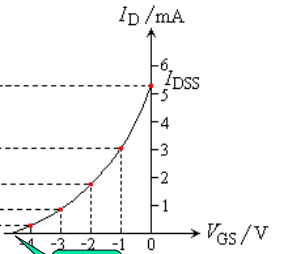
\includegraphics[]{01/结型场效应管转移特性曲线.png}

	特性和参数 :
	\begin{itemize}[leftmargin = 4em]
		\item 放大时, N沟道JEFT : gs为反偏压(g的点位比s低), ds为正偏压; P沟道相反
		\item 夹断电压 $ U_{P} $ : 漏极电流约为0时对应的 $ U_{GS} $
		\item 饱和漏极电流 $ I_{DSS} $ : $ U_{GS} = 0 $ 时对应的漏极电流
		\item 低频跨导 $ g_{m} $ : 相当于BJT的 $ \beta $, 单位是毫西门子(mS)
		\item 输出电阻 $ r_{ds} $ : 直流输入电阻 $ R_{GS} $
		\item 开启电压 $ U_{T} $ : 增强型绝缘栅型场效应管的参数, 栅源电压小于开启电压时, 场效应管不能导通
		\item 在饱和区时, $ i_{d} = I_{DSS}(1-\frac{u_{GS}}{U_{P}})^{2} $
	\end{itemize}

\end{document}